\documentclass[aspectratio=169,11pt]{beamer}

\usepackage[utf8]{inputenc}
\usepackage[T1]{fontenc}
\usepackage[spanish]{babel}
\usepackage{booktabs}
\usepackage{array}
\usepackage{graphicx}
\usepackage{xcolor}
\usepackage{amssymb}

\graphicspath{{Paper/figures/}{figures/}}

\definecolor{cjcblue}{HTML}{1F5EA8}
\definecolor{cjcyellow}{HTML}{F2C400}
\definecolor{cjcgray}{HTML}{4A4A4A}
\definecolor{cjclight}{HTML}{F5F6F7}
\definecolor{cjcpositive}{HTML}{4F81BD}
\definecolor{cjcnegative}{HTML}{C44E52}
\definecolor{cjcgold}{HTML}{B07800}

\usetheme{default}
\setbeamertemplate{navigation symbols}{}
\setbeamertemplate{footline}{
  \leavevmode%
  \hbox{%
    \begin{beamercolorbox}[wd=.78\paperwidth,ht=2.4ex,dp=1.1ex,leftskip=1.5em]{author in head/foot}%
      \scriptsize Centro Javeriano de Competitividad
    \end{beamercolorbox}%
    \begin{beamercolorbox}[wd=.22\paperwidth,ht=2.4ex,dp=1.1ex,rightskip=1.5em plus1fil]{date in head/foot}%
      \scriptsize \insertframenumber/\inserttotalframenumber
    \end{beamercolorbox}}%
  \vskip0pt%
}

\setbeamercolor{frametitle}{fg=cjcblue}
\setbeamercolor{title}{fg=cjcblue}
\setbeamercolor{normal text}{fg=black,bg=white}
\setbeamercolor{author in head/foot}{fg=white,bg=cjcblue}
\setbeamercolor{date in head/foot}{fg=white,bg=cjcgray}
\setbeamercolor{block title}{fg=cjcblue,bg=cjclight}
\setbeamercolor{block body}{fg=black,bg=cjclight}
\setbeamerfont{frametitle}{series=\bfseries,size=\large}
\setbeamerfont{title}{series=\bfseries,size=\LARGE}
\setbeamertemplate{itemize item}{\color{cjcblue}$\blacktriangleright$}
\setbeamertemplate{itemize subitem}{\color{cjcblue}$\bullet$}

\newcommand{\fuente}[1]{\vspace{0.10cm}{\tiny\color{cjcgray}#1}}
\newcommand{\idea}[1]{\textbf{\color{cjcblue}#1}}
\newcommand{\cjcbar}{\textcolor{cjcyellow}{\rule{0.18\textwidth}{1.6pt}}\hspace{0.3em}\textcolor{cjcblue}{\rule{0.72\textwidth}{1.6pt}}}
\newcommand{\pp}{\text{ pp}}

\title{La Productividad Total de los Factores por Actividad Económica en Colombia}
\subtitle{Informes sobre la Productividad en Colombia \\ Informe 02}
\author{Oliver Pardo \and Jorge Orozco}
\institute{Centro Javeriano de Competitividad}
\date{Julio de 2026}

\begin{document}

\begin{frame}[plain]
  \vspace{0.3cm}
  
\includegraphics[height=1.45cm]{logo_cjc_palatino_horizontal.png}

  \vspace{0.8cm}
  {\Large\color{cjcgray}Informes sobre la Productividad en Colombia}\\[0.2cm]
  {\large\color{cjcgray}Informe 02}\\[0.35cm]
  \cjcbar

  \vspace{0.75cm}
  {\LARGE\bfseries\color{cjcblue} La Productividad Total de los Factores por Actividad Económica en Colombia}

  \vspace{0.25cm}
  {\large\color{cjcgray}Avances y retrocesos, 2005--2025}

  \vfill
  {\large Oliver Pardo \quad | \quad Jorge Orozco}\\[0.15cm]
  {\normalsize Julio de 2026}
\end{frame}

\begin{frame}{Qué mide la Productividad Total de los Factores}
  \idea{La PTF es la parte del crecimiento de la economía que no se explica por la acumulación de capital físico o humano.}

  \vspace{0.35cm}
  \begin{block}{}
    \[
      \text{Crecimiento de la economía}
      =
      \text{aporte del capital físico y humano}
      +
      \text{PTF}
    \]
  \end{block}

  \vspace{0.25cm}
  \begin{columns}[T,totalwidth=\textwidth]
    \begin{column}{0.31\textwidth}
      \centering
      {\large\bfseries\color{cjcpositive}PTF positiva}\\[0.14cm]
      {\small La producción crece más de lo que explica la acumulación de factores.}
    \end{column}
    \begin{column}{0.31\textwidth}
      \centering
      {\large\bfseries\color{cjcgray}PTF igual a cero}\\[0.14cm]
      {\small El crecimiento se explica completamente por la acumulación de factores.}
    \end{column}
    \begin{column}{0.31\textwidth}
      \centering
      {\large\bfseries\color{cjcnegative}PTF negativa}\\[0.14cm]
      {\small El crecimiento es inferior al aporte estimado de los factores.}
    \end{column}
  \end{columns}

  \vfill
%  {\scriptsize\color{cjcgray}\textit{La PTF no es un factor adicional. El cálculo muestra cuánto aporta al crecimiento, pero no identifica por qué cambia.}}
\end{frame}

\begin{frame}{Por qué importa la PTF}
  \idea{Una mayor PTF permite que la economía crezca más sin aumentar al mismo ritmo el capital físico o humano.}

  \vspace{0.55cm}
  \begin{columns}[c,totalwidth=\textwidth]
    \begin{column}{0.27\textwidth}
      \centering
      {\Huge\bfseries\color{cjcgray}3,39\%}\\[0.12cm]
      {\small Crecimiento anual observado}
    \end{column}
    \begin{column}{0.08\textwidth}
      \centering
      {\Huge\bfseries\color{cjcblue}$\rightarrow$}
    \end{column}
    \begin{column}{0.28\textwidth}
      \centering
      {\Huge\bfseries\color{cjcgold}+1,00 pp}\\[0.12cm]
      {\small Crecimiento adicional de la PTF}
    \end{column}
    \begin{column}{0.08\textwidth}
      \centering
      {\Huge\bfseries\color{cjcblue}$\rightarrow$}
    \end{column}
    \begin{column}{0.27\textwidth}
      \centering
      {\Huge\bfseries\color{cjcblue}4,39\%}\\[0.12cm]
      {\small Crecimiento anual contrafactual}
    \end{column}
  \end{columns}

  \vspace{0.65cm}
  \begin{center}
    {\Huge\bfseries\color{cjcblue}23,4\% más}\\[0.18cm]
    {\large habría producido la economía en 2025}
  \end{center}

  \vfill
%  {\scriptsize\color{cjcgray}\textit{El ejercicio no supone más capital físico ni humano: atribuye toda la diferencia a una PTF más alta. Es un contrafactual contable, no una estimación causal.}}
\end{frame}

%\begin{comment}
%\begin{frame}{Cómo calcula el DANE la PTF}
%  \idea{El DANE atribuye primero parte del crecimiento a los recursos utilizados. La parte restante corresponde a la PTF.}

%  \vspace{0.25cm}
%  \begin{block}{Identidad contable}
%    \[
%      \text{Crecimiento de la producción}
%      -
%      \text{contribución de factores e insumos}
%      =
%      \text{PTF}
%    \]
%  \end{block}

%  \vspace{0.25cm}
%  \begin{columns}[T,totalwidth=\textwidth]
%    \begin{column}{0.47\textwidth}
%      {\large\bfseries\color{cjcblue}Enfoque de valor agregado}
%      \vspace{0.15cm}
%      \begin{itemize}
%        \item Total de la economía, 2005--2025.
%        \item Descuenta las contribuciones del trabajo y el capital.
%      \end{itemize}
%    \end{column}
%    \begin{column}{0.47\textwidth}
%      {\large\bfseries\color{cjcblue}Enfoque de producción}
    %  \vspace{0.15cm}
   %   \begin{itemize}
  %      \item Total y nueve ramas que abarcan toda la economía, 2005--2024.
 %       \item Descuenta trabajo, capital, energía, materiales y servicios.
 %     \end{itemize}
%    \end{column}
%  \end{columns}

%  \vfill
%  {\scriptsize\color{cjcgray}\textit{Los dos enfoques producen resultados distintos porque descuentan insumos distintos.}}
%\end{frame}
%\end{comment}

\begin{frame}{La PTF cayó en las últimas dos décadas}
  \idea{La PTF disminuyó un 2,8\% entre 2005 y 2025, equivalente a $-0,14$\% por año.}

  \vspace{0.10cm}
  \begin{center}
    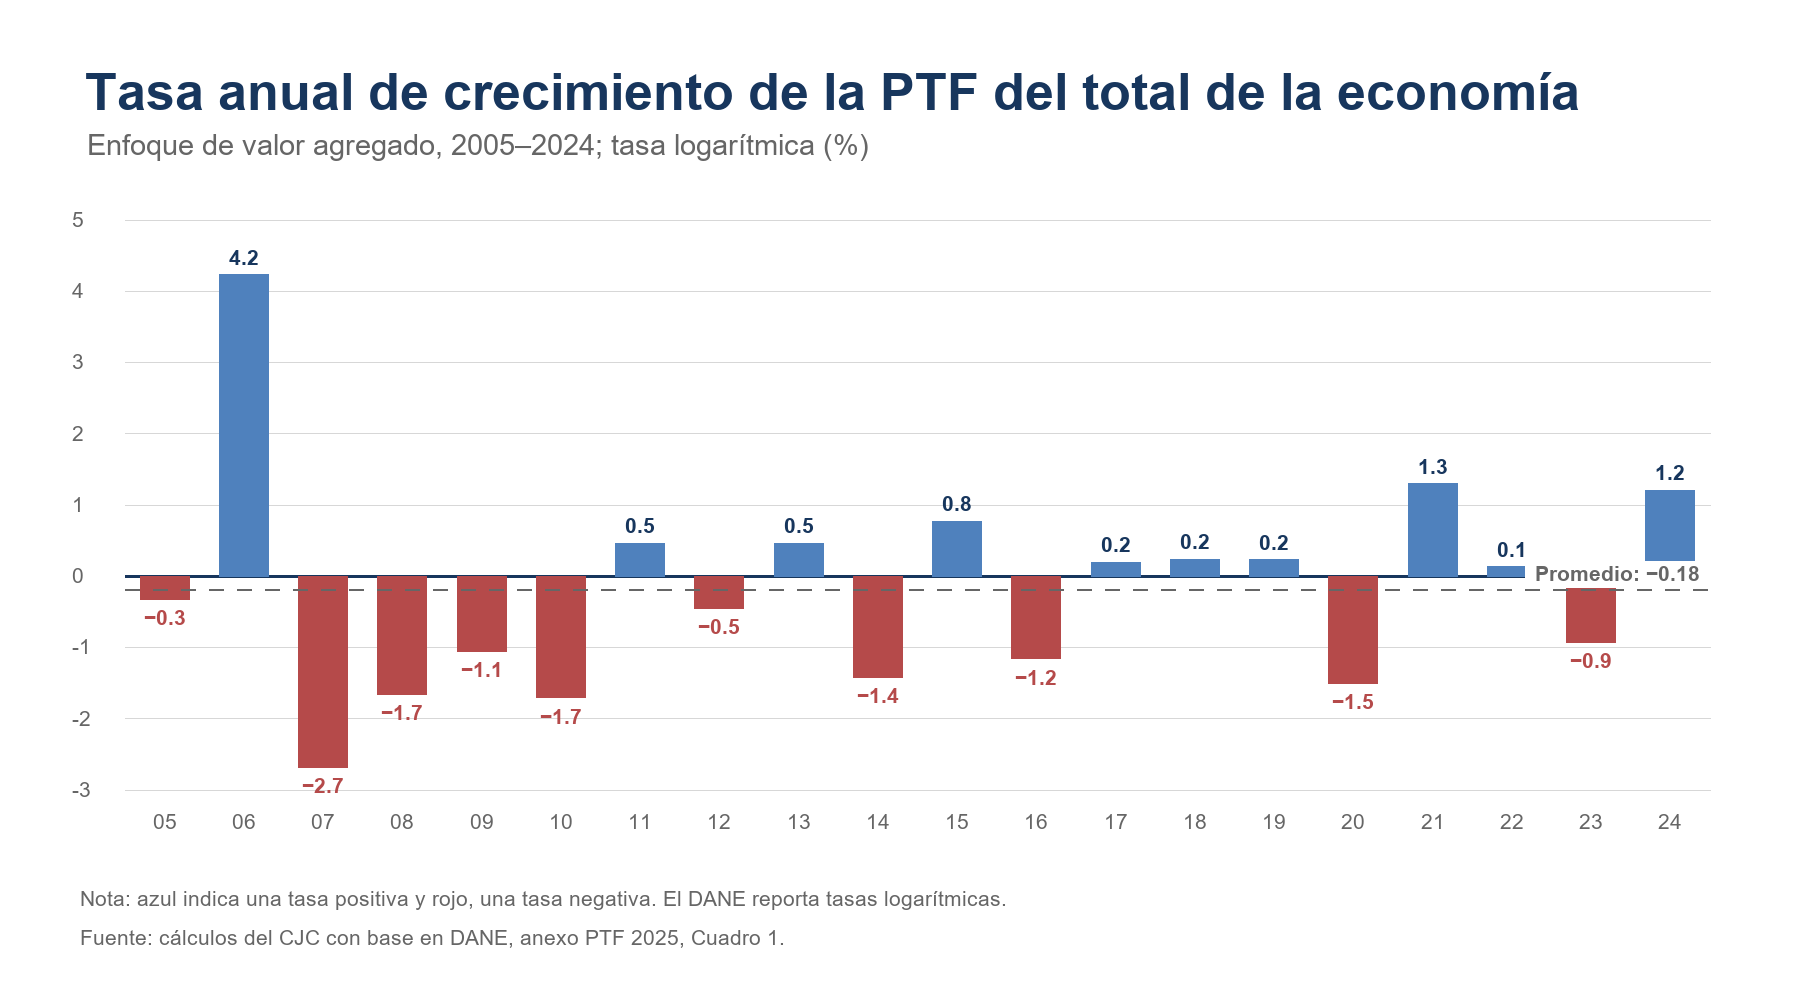
\includegraphics[width=0.94\textwidth,height=0.70\textheight,keepaspectratio]{fig_ptf_total_anual_valor_agregado.png}
  \end{center}
\end{frame}


\begin{frame}{La PTF total terminó por debajo de su nivel de 2005}
%  \idea{Al encadenar las tasas anuales de 2005 a 2024, el índice de la PTF pasó de 100 a 98,5.}

  \vspace{0.10cm}
  \begin{center}
    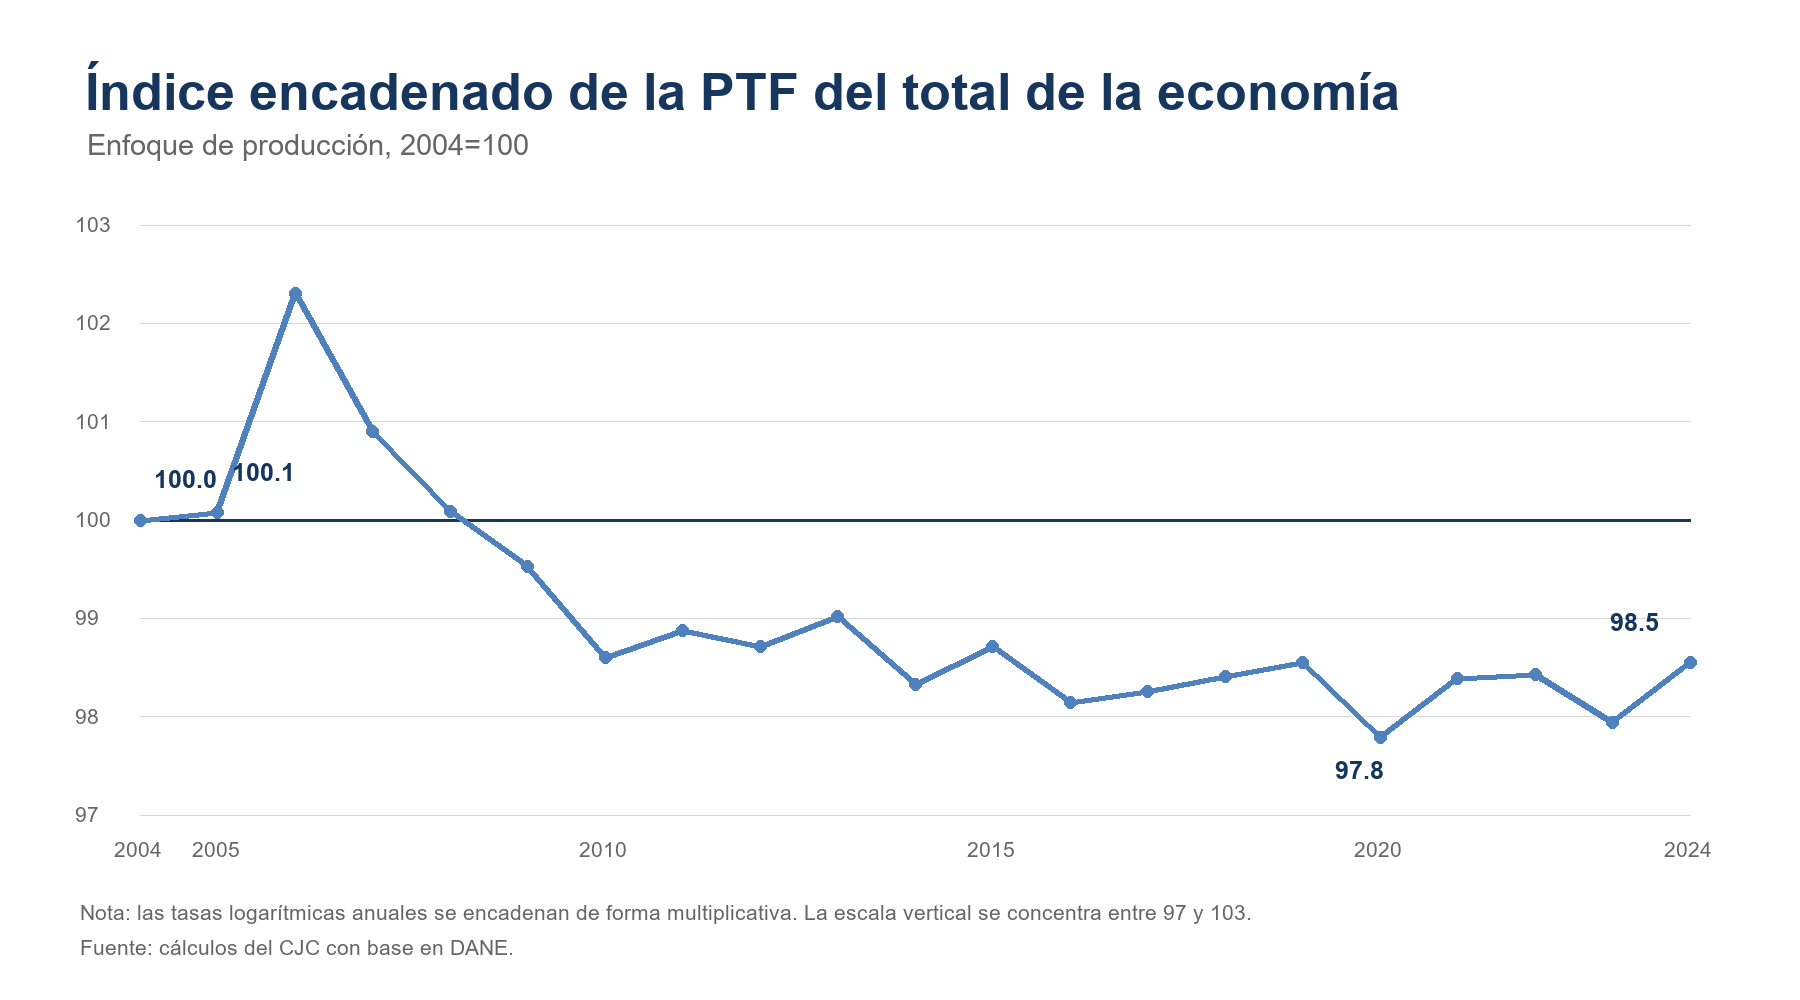
\includegraphics[width=0.92\textwidth,height=0.70\textheight,keepaspectratio]{fig_ptf_total_encadenada.png}
  \end{center}
\end{frame}


\begin{frame}{El crecimiento dependió del trabajo y el capital}
  \idea{Entre 2005 y 2025, el trabajo aportó 1,73 puntos porcentuales por año; el capital, 1,79; y la PTF restó 0,14.}

  \vspace{0.10cm}
  \begin{center}
    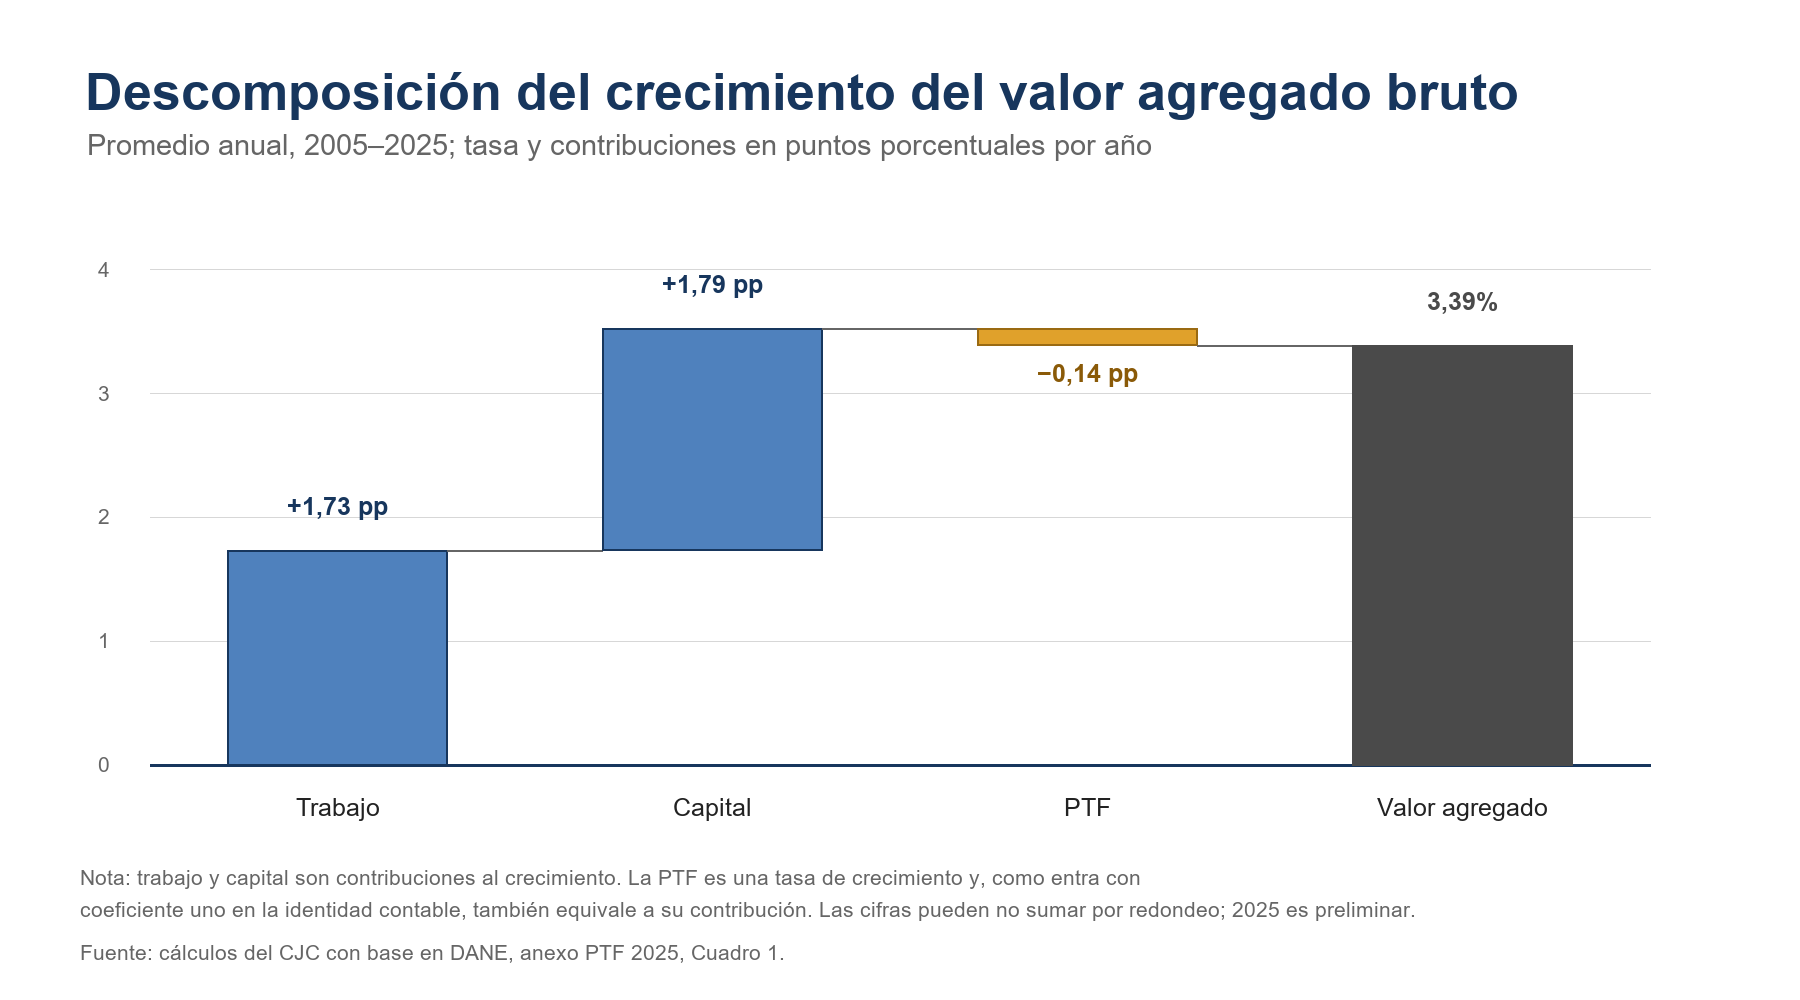
\includegraphics[width=0.92\textwidth,height=0.70\textheight,keepaspectratio]{fig_descomposicion_valor_agregado.png}
  \end{center}
\end{frame}

\begin{frame}{La PTF no evolucionó igual en todas las actividades}
  \idea{El estancamiento de la PTF total oculta trayectorias muy distintas entre las nueve ramas que abarcan toda la economía.}

  \vspace{0.05cm}
  \begin{center}
    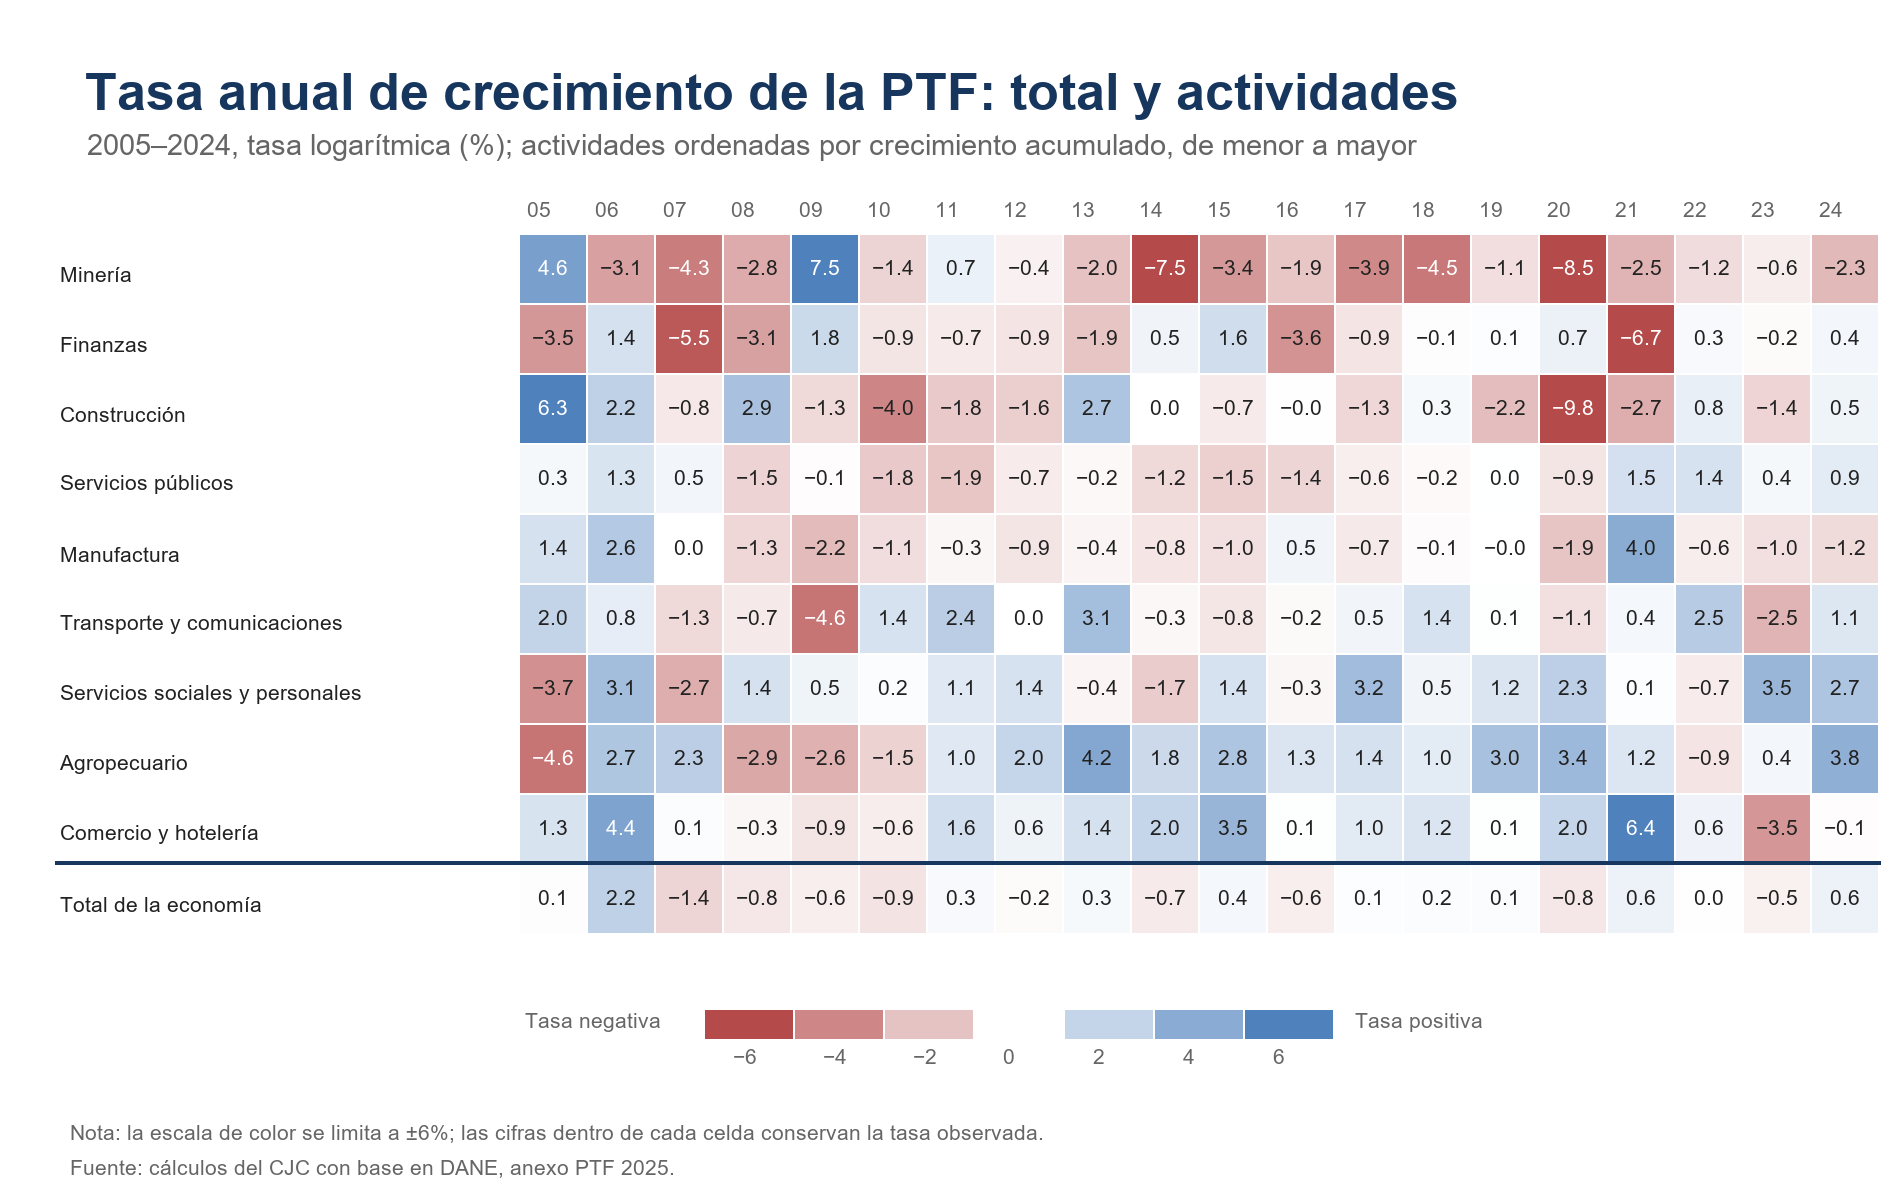
\includegraphics[width=0.98\textwidth,height=0.72\textheight,keepaspectratio]{fig_ptf_mapa_anual.png}
  \end{center}
\end{frame}

\begin{frame}{Cuatro ramas avanzaron y cinco retrocedieron}
  \idea{Entre 2005 y 2024, la PTF de comercio y hotelería aumentó 23,2\%, mientras la de minería disminuyó 32,1\%.}

  \vspace{0.05cm}
  \begin{center}
    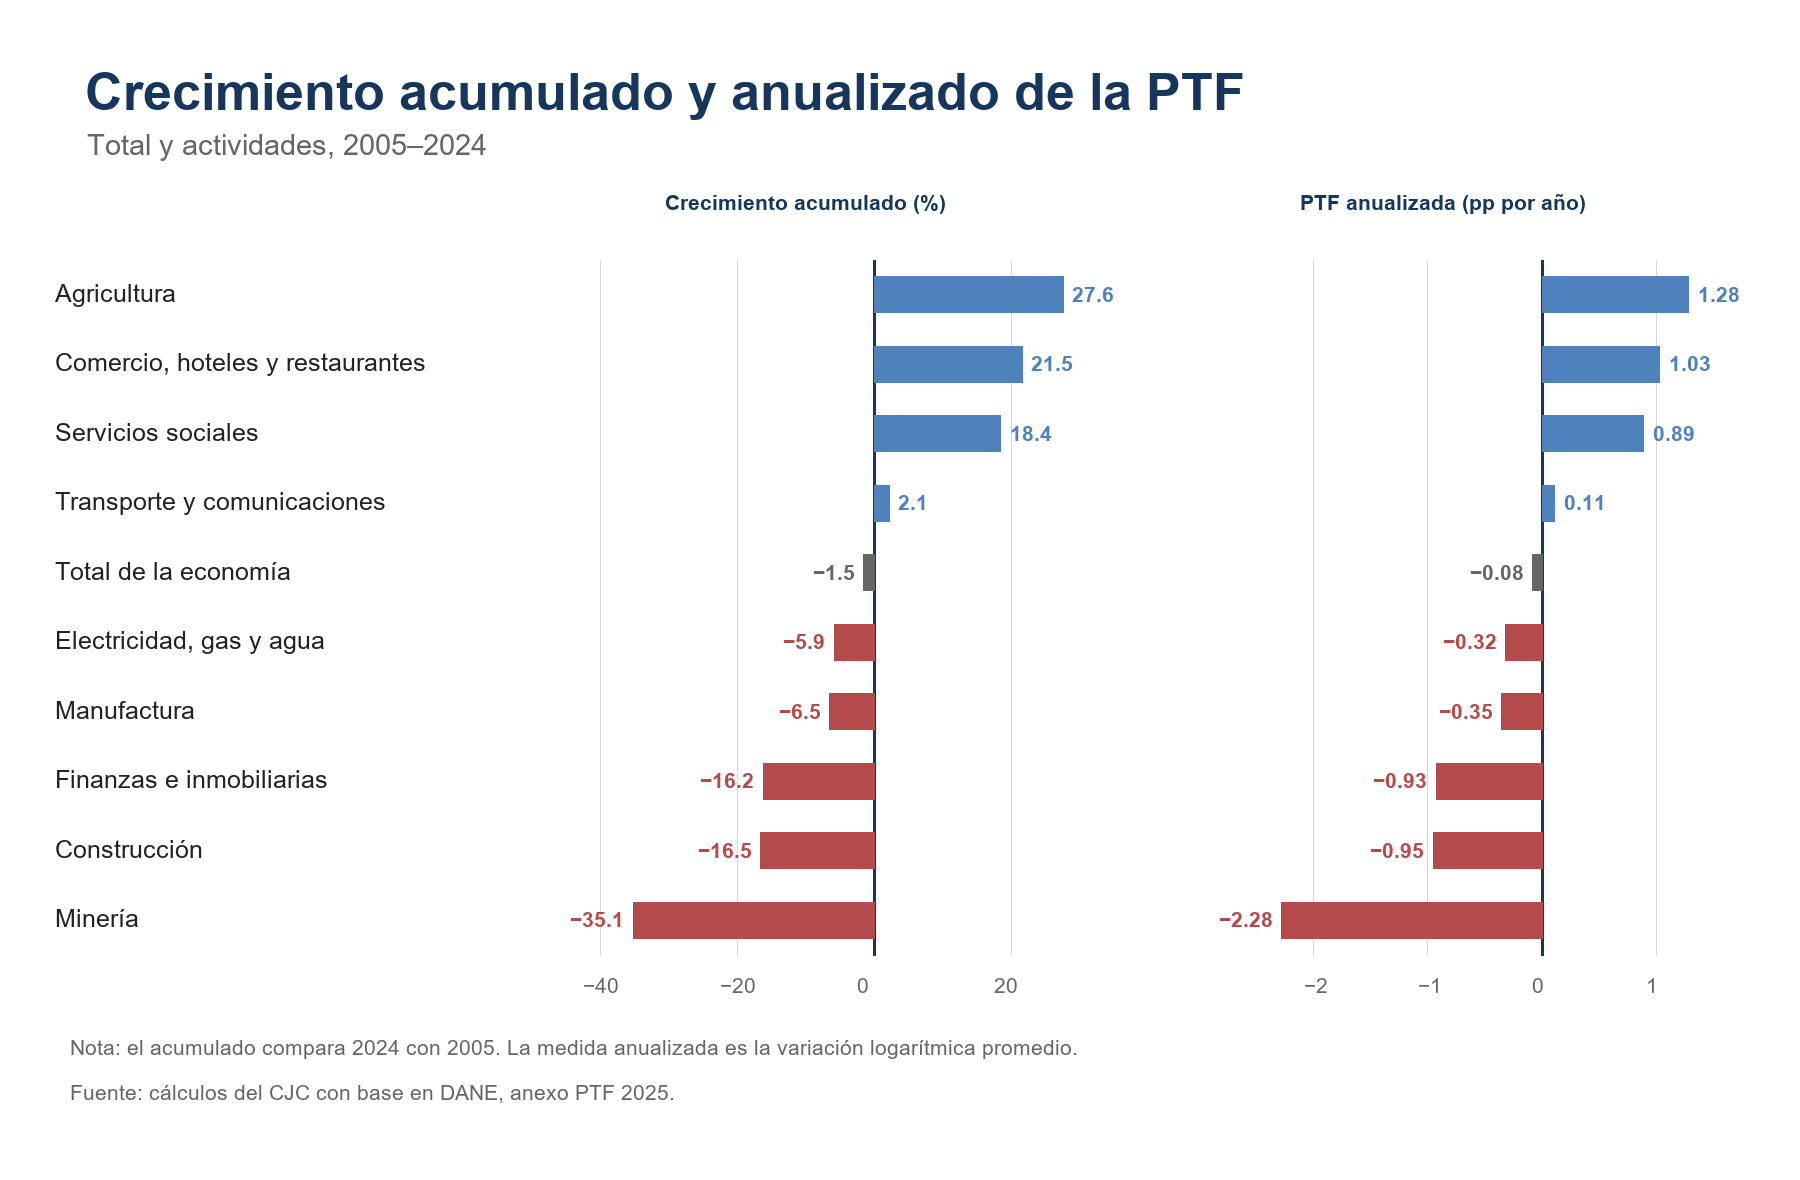
\includegraphics[width=0.98\textwidth,height=0.72\textheight,keepaspectratio]{fig_ptf_promedio_actividad.png}
  \end{center}
\end{frame}

%\begin{frame}{El efecto agregado depende del crecimiento y del peso de cada rama}
 % \idea{La contribución de cada rama depende de la tasa de crecimiento de su PTF y de su participación anual en la producción nominal.}

  %\vspace{0.18cm}
  %\begin{center}
  %\scriptsize
  %\setlength{\tabcolsep}{3.1pt}
  %\begin{tabular}{@{}lrrrr@{}}
   % \toprule
    %Actividad & Peso promedio & PTF acumulada & PTF anualizada & Contribución anual \\
    %\midrule
    %Comercio y hotelería & 12,98\% & 23,17\% & 1,04\% & 0,13 pp \\
    %Agropecuario & 6,11\% & 21,84\% & 0,99\% & 0,06 pp \\
    %Servicios sociales y personales & 16,05\% & 14,16\% & 0,66\% & 0,11 pp \\
    %Transporte y comunicaciones & 8,63\% & 4,26\% & 0,21\% & 0,02 pp \\
    %Manufactura & 23,43\% & $-5,15$\% & $-0,26$\% & $-0,06$ pp \\
    %Servicios públicos & 3,42\% & $-5,53$\% & $-0,28$\% & $-0,01$ pp \\
    %Construcción & 8,64\% & $-11,06$\% & $-0,59$\% & $-0,05$ pp \\
    %Financieras & 14,66\% & $-19,01$\% & $-1,05$\% & $-0,15$ pp \\
    %Minería & 6,08\% & $-32,09$\% & $-1,93$\% & $-0,11$ pp \\
    %\midrule
    %\textbf{Total de la economía} & %\textbf{100,00\%} & \textbf{$-1,45$\%} & %\textbf{$-0,07$\%} & \textbf{$-0,07$ pp} %\\
%    \bottomrule
%  \end{tabular}
%  \end{center}

%  \fuente{Fuente: cálculos del CJC con base en DANE.}
%\end{frame}

\begin{frame}{Contribuciones al crecimiento}
  \idea{Cuatro ramas sumaron 0,32 puntos porcentuales por año al crecimiento de la PTF total; cinco restaron 0,39.}

  \vspace{0.05cm}
  \begin{center}
    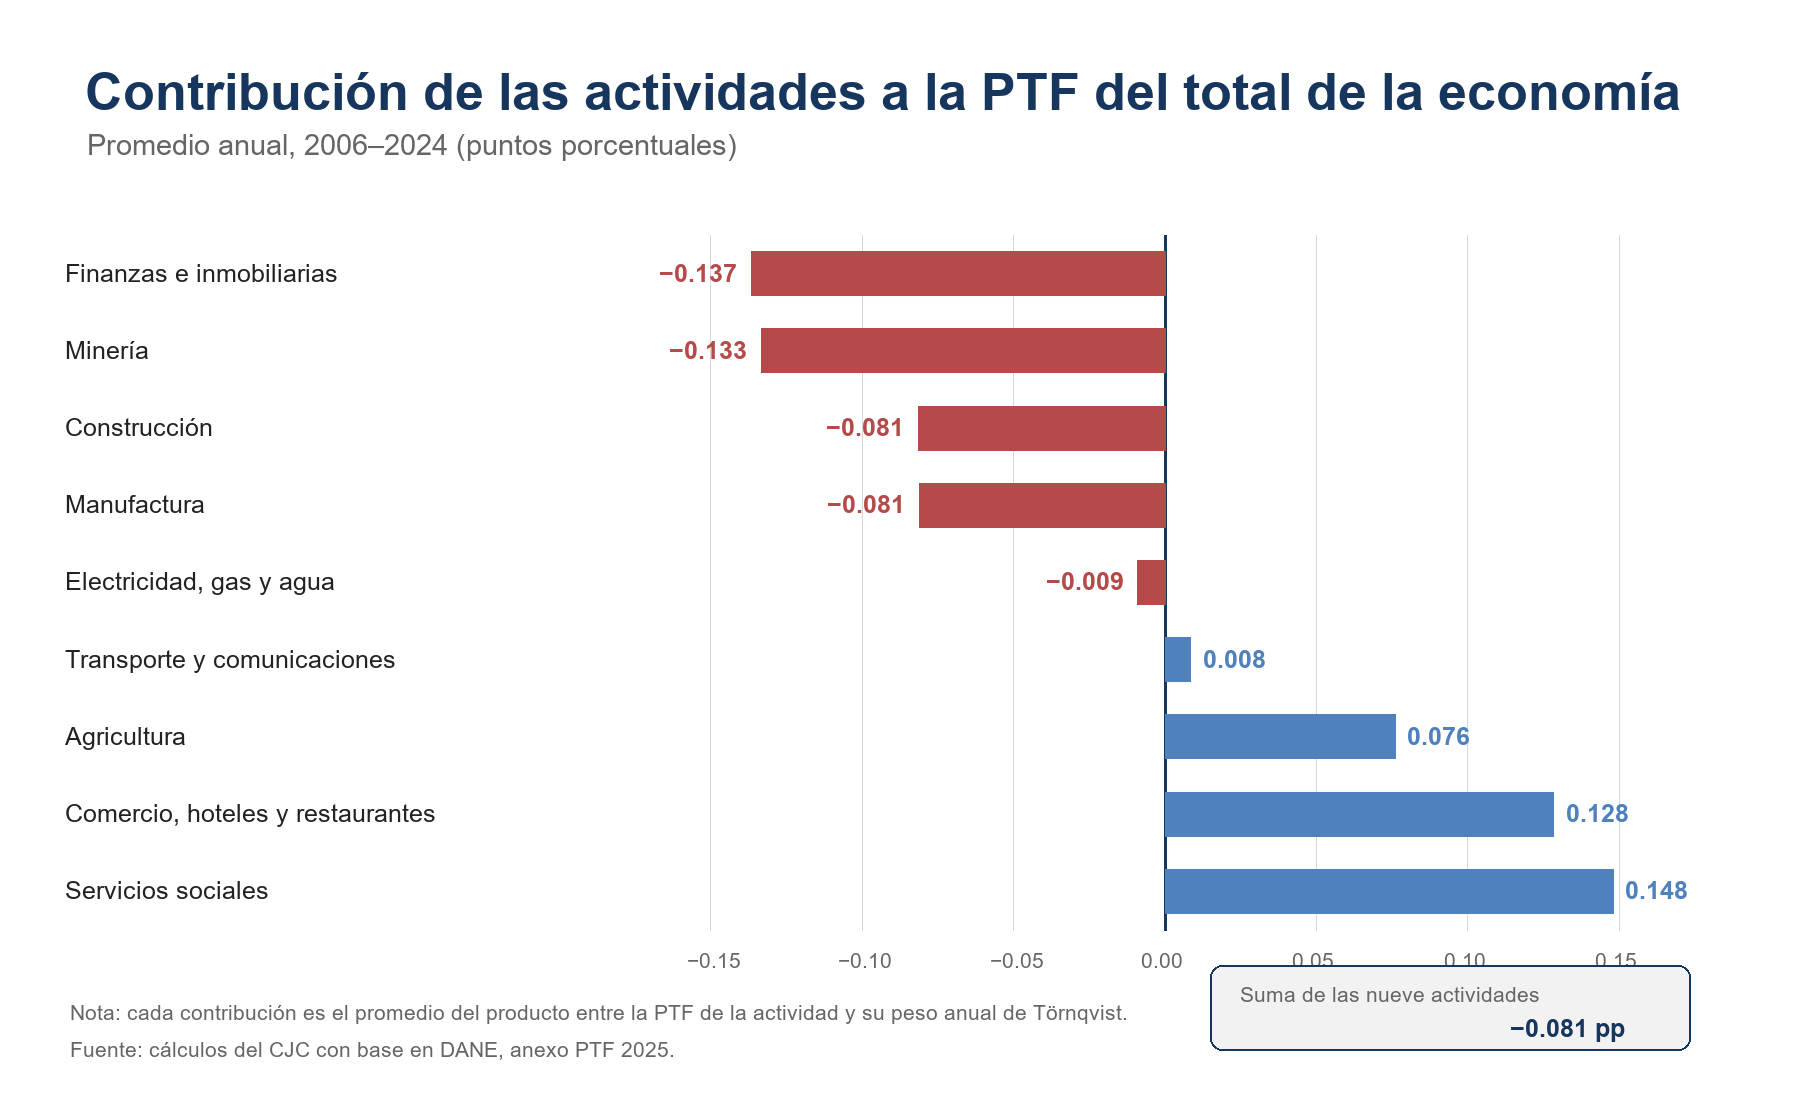
\includegraphics[width=0.98\textwidth,height=0.72\textheight,keepaspectratio]{fig_ptf_contribucion_total_actividad.png}
  \end{center}
\end{frame}


\begin{frame}{Descomposición del crecimiento de las ramas de actividad}
  \idea{El uso de factores e insumos impulsó la producción de todas las ramas, aunque la caída de la PTF contrarrestó parte de ese aporte en cinco ramas.}

  \vspace{0.05cm}
  \begin{center}
    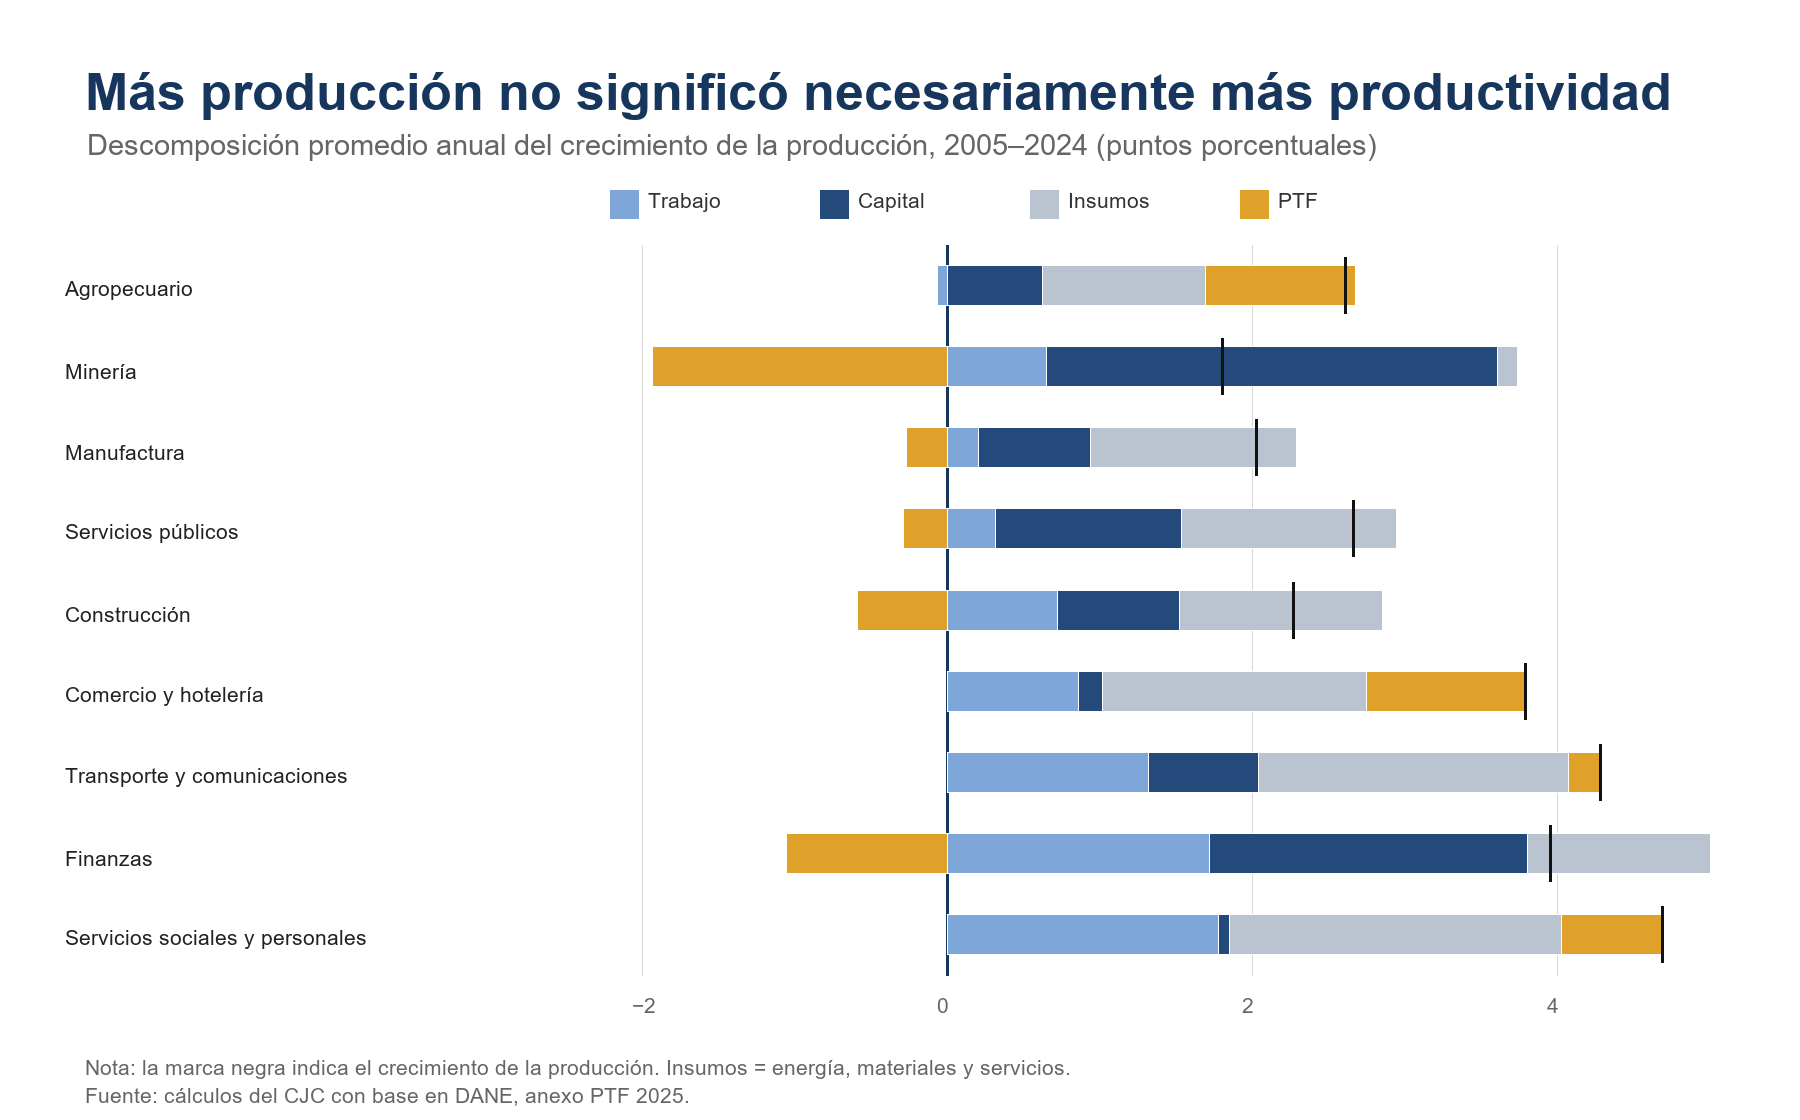
\includegraphics[width=0.98\textwidth,height=0.72\textheight,keepaspectratio]{fig_descomposicion_actividad.png}
  \end{center}
\end{frame}

\begin{frame}{Aportes a la tasa de crecimiento}
  \idea{Sin las contribuciones negativas de cinco ramas, la economía habría crecido 3,65\% anual en lugar de 3,26\%.}

  \vspace{0.05cm}
  \begin{center}
    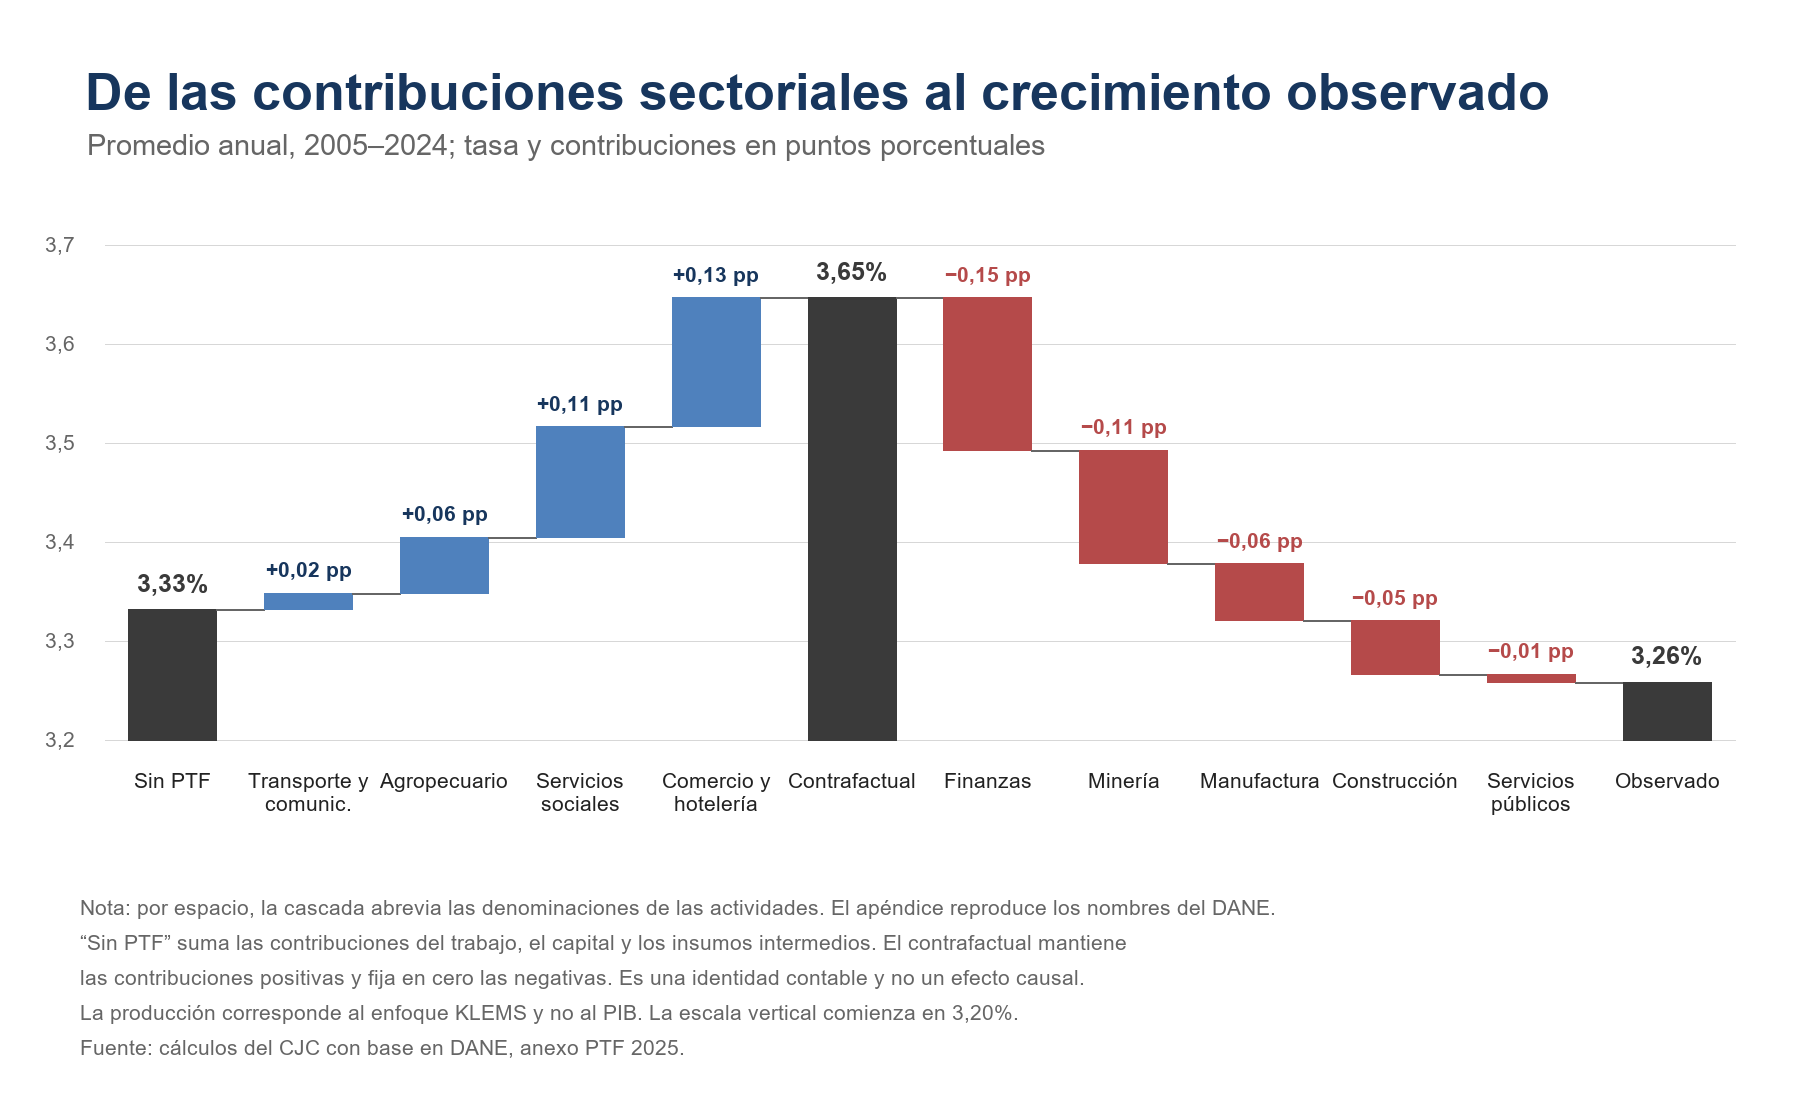
\includegraphics[width=0.94\textwidth,height=0.72\textheight,keepaspectratio]{fig_ptf_cascada_contribuciones_actividad.png}
  \end{center}
\end{frame}

\begin{frame}{Conclusiones}
  \idea{La política de productividad debe empezar por identificar por qué cayó la PTF en las actividades que más redujeron el crecimiento.}

  \vspace{0.30cm}
  \begin{itemize}
    \item La PTF de la economía colombiana estuvo estancada durante al menos las últimas dos décadas.
    \item El resultado total no fue común a toda la economía: la PTF aumentó en cuatro de las nueve ramas y disminuyó en cinco.
    \item Las caídas de la PTF en las actividades financieras, la minería, la manufactura y la construcción restaron 0,4 puntos porcentuales por año al crecimiento de la economía.
    %\item Los datos muestran cuánto aportó o restó la PTF de cada rama, pero no establecen por qué aumentó o disminuyó.
    \item Si el país quiere acelerar su crecimiento, debe identificar los obstáculos que explican las caídas de la PTF en al menos esas cuatro actividades.
  \end{itemize}
\end{frame}

\begin{frame}{Apéndice: qué incluye cada rama de actividad}
  \idea{Las nueve ramas corresponden a la mayor desagregación sectorial de la PTF que publica el DANE.}

  \vspace{0.18cm}
  \begin{center}
  \scriptsize
  \setlength{\tabcolsep}{4pt}
  \begin{tabular}{@{}>{\raggedright\arraybackslash}p{3.0cm}>{\raggedright\arraybackslash}p{10.5cm}@{}}
    \toprule
    Rama & Subactividades incluidas \\
    \midrule
    Agropecuario & Agricultura, ganadería, caza, silvicultura y pesca. \\
    \addlinespace
    Minería & Explotación de minas y canteras. \\
    \addlinespace
    Manufactura & Alimentos, textiles, refinación, químicos, metales, maquinaria, equipo y otras manufacturas. \\
    \addlinespace
    Servicios públicos & Suministro de electricidad, gas y agua. \\
    \addlinespace
    Construcción & Construcción. \\
    \bottomrule
  \end{tabular}
  \end{center}

  \fuente{Fuente: DANE.}
\end{frame}

\begin{frame}{Apéndice: las ramas de servicios agrupan actividades heterogéneas}
  \idea{Las categorías permiten comparar toda la economía, pero no identificar resultados por subactividad.}

  \vspace{0.18cm}
  \begin{center}
  \scriptsize
  \setlength{\tabcolsep}{4pt}
  \begin{tabular}{@{}>{\raggedright\arraybackslash}p{3.2cm}>{\raggedright\arraybackslash}p{10.3cm}@{}}
    \toprule
    Rama & Subactividades incluidas \\
    \midrule
    Comercio y hotelería & Comercio, reparación de vehículos, hoteles y restaurantes. \\
    \addlinespace
    Transporte y comunicaciones & Transporte, almacenamiento y comunicaciones. \\
    \addlinespace
    Financieras & Intermediación financiera; actividades inmobiliarias, empresariales y de alquiler. \\
    \addlinespace
    Servicios sociales y personales & Administración pública, educación, salud, servicios comunitarios y personales, hogares y organismos extraterritoriales. \\
    \bottomrule
  \end{tabular}
  \end{center}

  \fuente{Fuente: DANE.}
\end{frame}

\end{document}
